\documentclass[10pt,landscape]{article}
\usepackage[usenames,dvips,pdftex]{color}
\usepackage{multicol}
\usepackage{calc}
\usepackage{ifthen}
\usepackage[pdftex]{color,graphicx}
\usepackage[landscape]{geometry}
\usepackage{hyperref}
\hypersetup{colorlinks=true, filecolor=black, linkcolor=black, urlcolor=blue, citecolor=black}
\graphicspath{{./images/}}


% To make this come out properly in landscape mode, do one of the following
% 1.
%  pdflatex latexsheet.tex
%
% 2.
%  latex latexsheet.tex
%  dvips -P pdf  -t landscape latexsheet.dvi
%  ps2pdf latexsheet.ps


% If you're reading this, be prepared for confusion.  Making this was
% a learning experience for me, and it shows.  Much of the placement
% was hacked in; if you make it better, let me know...


% 2008-04
% Changed page margin code to use the geometry package. Also added code for
% conditional page margins, depending on paper size. Thanks to Uwe Ziegenhagen
% for the suggestions.

% 2006-08
% Made changes based on suggestions from Gene Cooperman. <gene at ccs.neu.edu>


% To Do:
% \listoffigures \listoftables
% \setcounter{secnumdepth}{0}


% This sets page margins to .5 inch if using letter paper, and to 1cm
% if using A4 paper. (This probably isn't strictly necessary.)
% If using another size paper, use default 1cm margins.
\ifthenelse{\lengthtest { \paperwidth = 11in}}
	{ \geometry{top=.40in,left=.5in,right=.5in,bottom=.40in} }
	{\ifthenelse{ \lengthtest{ \paperwidth = 297mm}}
		{\geometry{top=1cm,left=1cm,right=1cm,bottom=1cm} }
		{\geometry{top=1cm,left=1cm,right=1cm,bottom=1cm} }
	}

% Turn off header and footer
\pagestyle{empty}


% Redefine section commands to use less space
\makeatletter
\renewcommand{\section}{\@startsection{section}{1}{0mm}%
                                {-0mm} %plus -.5mm minus -.5mm}%
                                {0.5mm}%x
                                {\normalfont\large\bfseries}}
\renewcommand{\subsection}{\@startsection{subsection}{2}{0mm}%
                                {-0mm}%
                                {0.5ex plus .2ex}%
                                {\normalfont\normalsize\bfseries}}
\renewcommand{\subsubsection}{\@startsection{subsubsection}{3}{0mm}%
                                {-1mm}%
                                {1ex plus .2ex}%
                                {\normalfont\small\bfseries}}
\makeatother

% Define BibTeX command
\def\BibTeX{{\rm B\kern-.05em{\sc i\kern-.025em b}\kern-.08em
    T\kern-.1667em\lower.7ex\hbox{E}\kern-.125emX}}

% Don't print section numbers
\setcounter{secnumdepth}{0}


\setlength{\parindent}{0pt}
\setlength{\parskip}{0pt plus 0.5ex}


\newif\ifcatkin
\catkintrue

\newenvironment{nstabbing}
  {\setlength{\topsep}{1pt}%
   \setlength{\partopsep}{1pt}%
   \tabbing}
  {\endtabbing}

% -----------------------------------------------------------------------

\begin{document}

\raggedright
\footnotesize
\begin{multicols}{3}

\setlength{\premulticols}{1pt}
\setlength{\postmulticols}{1pt}
\setlength{\multicolsep}{1pt}
\setlength{\columnsep}{2pt}

\begin{center}
     \Large{\textbf{ROS Indigo Cheatsheet}} \\
\end{center}
\newlength{\MyLen}
\settowidth{\MyLen}{\texttt{letterpaper}/\texttt{a4paper} \ }

\vspace{-2mm}
\section{Filesystem Management Tools}
\begin{tabular}{@{}p{\the\MyLen}%
                @{}p{\linewidth-\the\MyLen}@{}}
\ifcatkin
\texttt{\href{http://wiki.ros.org/rospack}{rospack}} & A tool for inspecting \href{http://wiki.ros.org/Packages}{packages}. \\
\texttt{\href{http://docs.ros.org/independent/api/rospkg/html/rospack.html\#rospack-profile}{rospack profile}} & Fixes path and pluginlib problems. \\
\texttt{\href{http://wiki.ros.org/rosbash\#roscd}{roscd}} & Change directory to a package. \\
\else
\texttt{\href{http://wiki.ros.org/rospack}{rospack}}/\texttt{rosstack} & A tool inspecting \href{http://wiki.ros.org/Packages}{packages}. \\
\texttt{\href{http://docs.ros.org/independent/api/rospkg/html/rospack.html\#rospack-profile}{rospack profile}} & Fixes path and pluginlib problems. \\
\texttt{\href{http://wiki.ros.org/rosbash\#roscd}{roscd}} & Change directory to a package or stack. \\
\fi
\texttt{\href{http://wiki.ros.org/rosbash\#rospd}{rospd}}/\texttt{\href{http://wiki.ros.org/rosbash\#rosd}{rosd}} & \href{http://ftp.gnu.org/old-gnu/Manuals/bash-2.05a/html\_node/bashref\_73.html}{Pushd} equivalent for \href{http://wiki.ros.org/rosbash\#roscd}{ROS}. \\
\texttt{\href{http://wiki.ros.org/rosbash\#rosls}{rosls}} & Lists package or stack information. \\
\texttt{\href{http://wiki.ros.org/rosbash\#rosed}{rosed}} & Open requested ROS file in a text editor. \\
\texttt{\href{http://wiki.ros.org/rosbash\#roscp}{roscp}} & Copy a file from one place to another. \\
\texttt{\href{http://wiki.ros.org/rosdep}{rosdep}} & Installs package system dependencies.\\
\texttt{\href{http://wiki.ros.org/roswtf}{roswtf}} & Displays a errors and warnings about a running ROS system or launch file.\\
\ifcatkin
\texttt{\href{http://wiki.ros.org/catkin/Tutorials/CreatingPackage}{catkin\_create\_pkg}} & Creates a new ROS stack.\\
\texttt{\href{http://wiki.ros.org/wstool}{wstool}} & Manage many repos in workspace. \\
\texttt{\href{http://wiki.ros.org/catkin}{catkin\_make}} & Builds a ROS catkin workspace.\\
\else
\texttt{\href{http://wiki.ros.org/roscreate}{roscreate}-pkg} & Creates a new ROS package. \\
\texttt{\href{http://wiki.ros.org/roscreate}{roscreate}-stack} & Creates a new ROS stack.\\
\texttt{\href{http://wiki.ros.org/rosmake}{rosmake}} & Builds a ROS package.\\
\fi
\texttt{\href{http://wiki.ros.org/rqt\_dep}{rqt\_dep}} & Displays package structure and dependencies.\\
\end{tabular}

\begin{nstabbing}
Us\=age:\\
\> \texttt{\$ rospack find [package]}\\
\> \texttt{\$ roscd [package[/subdir]]}\\
\> \texttt{\$ rospd [package[/subdir] | +N | -N]}\\
\> \texttt{\$ rosd}\\
\> \texttt{\$ rosls [package[/subdir]]}\\
\> \texttt{\$ rosed [package] [file]}\\
\> \texttt{\$ roscp [package] [file] [destination]}\\
\> \texttt{\$ rosdep install [package]}\\
\> \texttt{\$ roswtf or roswtf [file]}\\
\ifcatkin
\> \texttt{\$ catkin\_create\_pkg [package\_name] [depend1]..[dependN]}\\
\> \texttt{\$ wstool [init | set | update]}\\
\> \texttt{\$ catkin\_make}\\
\else
\> \texttt{\$ roscreate-pkg [package\_name]}\\
\> \texttt{\$ rosmake [package]}\\
\fi
\> \texttt{\$ rqt\_dep [options]}\\
\end{nstabbing}

\vspace{-5mm}
\section{Start-up and Process Launch Tools}
\vspace{-2 mm}
\subsection{\href{http://wiki.ros.org/roscore}{roscore}}
The basis \href{http://wiki.ros.org/Nodes}{nodes} and programs for ROS-based systems. A roscore must be running for ROS nodes to communicate.\\
\begin{nstabbing}
Us\=age:\\
\> \texttt{\$ roscore}
\end{nstabbing}

\vspace{-2 mm}
\subsection{\href{http://wiki.ros.org/rosrun}{rosrun}}
Runs a ROS package's executable with minimal typing.\\
\begin{nstabbing}
Us\=age:\\
\> \texttt{\$ rosrun package\_name executable\_name}
\end{nstabbing}
\begin{nstabbing}
Ex\=ample (runs \href{http://wiki.ros.org/turtlesim}{turtlesim}):\\
\> \texttt{\$ rosrun turtlesim turtlesim\_node}\\
\end{nstabbing}
\vspace{-1 mm}

\subsection{\href{http://wiki.ros.org/roslaunch}{roslaunch}}
Starts a roscore (if needed), \href{http://wiki.ros.org/roslaunch/XML#Minimal_Example}{local nodes}, \href{http://wiki.ros.org/roslaunch/XML/machine}{remote nodes} via SSH, and sets parameter server \href{http://wiki.ros.org/roslaunch/XML#Setting_parameters}{parameters}.\\
\begin{nstabbing}
E\=x\=amples:\\
\> Launch a file in a package:\\
\> \> \texttt{\$ roslaunch package\_name file\_name.launch}\\
\> Launch on a different port:\\
\> \> \texttt{\$ roslaunch -p 1234 package\_name file\_name.launch}\\
\> Launch on the local nodes:\\
\> \> \texttt{\$ roslaunch --local package\_name file\_name.launch}
\end{nstabbing}


\section{Introspection and Command Tools}

\subsection{\href{http://wiki.ros.org/rosnode}{rosnode}}
Displays debugging information about ROS nodes, including publications, subscriptions and connections.\\
Commands: \\
\begin{tabular}{p{\the\MyLen}%
                @{}p{\linewidth-\the\MyLen}@{}}
\texttt{rosnode ping}    & Test connectivity to node. \\
\texttt{rosnode list}    & List active nodes. \\
\texttt{rosnode info}    & Print information about a node. \\
\texttt{rosnode machine} & List nodes running on a machine. \\
\texttt{rosnode kill}    & Kill a running node.
\end{tabular}
\begin{nstabbing}
E\=x\=amples:\\
\> Kill all nodes:\\
\> \> \texttt{\$ rosnode kill -a}\\
\> List nodes on a machine:\\
\> \> \texttt{\$ rosnode machine aqy.local}\\
\> Ping all nodes:\\
\> \> \texttt{\$ rosnode ping --all}
\end{nstabbing}


\subsection{\href{http://wiki.ros.org/rostopic}{rostopic}}
A tool for displaying information about ROS \href{http://wiki.ros.org/Topics}{topics}, including publishers, subscribers, publishing rate, and messages.\\
Commands: \\
\begin{tabular}{p{\the\MyLen}%
                @{}p{\linewidth-\the\MyLen}@{}}
\texttt{rostopic bw}     & Display bandwidth used by topic. \\
\texttt{rostopic echo}   & Print messages to screen. \\
\texttt{rostopic find}   & Find topics by type. \\
\texttt{rostopic hz}     & Display publishing rate of topic. \\
\texttt{rostopic info}   & Print information about an active topic. \\
\texttt{rostopic list}   & List all published topics. \\
\texttt{rostopic pub}    & Publish data to topic. \\
\texttt{rostopic type}   & Print topic type. \\
\end{tabular}
\begin{nstabbing}
E\=x\=amples:\\
\> Publish hello at 10 Hz:\\
\> \>\texttt{\$ rostopic pub -r 10 /topic\_name std\_msgs/String hello}\\
\> Clear the screen after each message is published:\\
\> \>\texttt{\$ rostopic echo -c /topic\_name}\\
\> Display messages that match a given Python expression:\\
\> \>\texttt{\$ rostopic echo --filter "m.data=='foo'"  /topic\_name}\\
\> Pipe the output of rostopic to rosmsg to view the msg type:\\
\> \>\texttt{\$ rostopic type /topic\_name | rosmsg show}
\end{nstabbing}

\subsection{\href{http://wiki.ros.org/rosservice}{rosservice}}
A tool for listing and querying ROS services.\\
Commands: \\
\begin{tabular}{p{\the\MyLen}%
                @{}p{\linewidth-\the\MyLen}@{}}
\texttt{rosservice list}  & Print information about active services. \\
\texttt{rosservice node}  & Print name of node providing a service. \\
\texttt{rosservice call}  & Call the service with the given args. \\
\texttt{rosservice args}  & List the arguments of a service. \\
\texttt{rosservice type}  & Print the service type. \\
\texttt{rosservice uri}   & Print the service ROSRPC uri. \\
\texttt{rosservice find}  & Find services by service type.
\end{tabular}
\begin{nstabbing}
E\=x\=amples:\\
\> Call a service from the command-line:\\
\> \>\texttt{\$ rosservice call /add\_two\_ints 1 2}\\
\> Pipe the output of rosservice to rossrv to view the srv type:\\
\> \>\texttt{\$ rosservice type add\_two\_ints | rossrv show}\\
\> Display all services of a particular type:\\
\> \>\texttt{\$ rosservice find rospy\_tutorials/AddTwoInts}\\
\end{nstabbing}

\subsection{\href{http://wiki.ros.org/rosparam}{rosparam}}
A tool for getting and setting ROS \href{http://wiki.ros.org/Parameter Server}{parameters} on the parameter server using YAML-encoded files.\\
Commands: \\
\begin{tabular}{p{\the\MyLen}%
                @{}p{\linewidth-\the\MyLen}@{}}
\texttt{rosparam set}    & Set a parameter. \\
\texttt{rosparam get}    & Get a parameter. \\
\texttt{rosparam load}   & Load parameters from a file. \\
\texttt{rosparam dump}   & Dump parameters to a file. \\
\texttt{rosparam delete} & Delete a parameter. \\
\texttt{rosparam list}   & List parameter names.
\end{tabular}
\begin{nstabbing}
E\=x\=amples:\\
\> List all the parameters in a namespace:\\
\> \>\texttt{\$ rosparam list /namespace}\\
\> Setting a list with one as a string, integer, and float:\\
\> \>\texttt{\$ rosparam set /foo "['1', 1, 1.0]"}\\
\> Dump only the parameters in a specific namespace to file:\\
\> \>\texttt{\$ rosparam dump dump.yaml /namespace}
\end{nstabbing}

\subsection{\href{http://wiki.ros.org/rosmsg}{rosmsg/rossrv}}
Displays Message/Service (msg/srv) data structure definitions.\\
Commands: \\
\begin{tabular}{p{\the\MyLen}%
                @{}p{\linewidth-\the\MyLen}@{}}
\texttt{rosmsg show}    & Display the fields in the msg/srv. \\
\texttt{rosmsg list}    & Display names of all msg/srv. \\
\texttt{rosmsg md5}    & Display the msg/srv md5 sum. \\
\texttt{rosmsg package} & List all the msg/srv in a package. \\
\texttt{rosmsg packages}    & List all packages containing the msg/srv.
\end{tabular}
\begin{nstabbing}
E\=x\=amples:\\
\> Display the Pose msg:\\
\> \> \texttt{\$ rosmsg show Pose}\\
\> List the messages in the nav\_msgs package:\\
\> \> \texttt{\$ rosmsg package nav\_msgs}\\
\> List the packages using sensor\_msgs/CameraInfo:\\
\> \> \texttt{\$ rosmsg packages sensor\_msgs/CameraInfo}
\end{nstabbing}

\section{Logging Tools}
\subsection{\href{http://wiki.ros.org/rosbag}{rosbag}}
A set of tools for recording and playing back of ROS topics.\\
Commands: \\
\begin{tabular}{p{\the\MyLen}%
                @{}p{\linewidth-\the\MyLen}@{}}
\texttt{rosbag record}  & Record a bag file with specified topics. \\
\texttt{rosbag play}  & Play content of one or more bag files. \\
\texttt{rosbag compress}  & Compress one or more bag files. \\
\texttt{rosbag decompress}  & Decompress one or more bag files. \\
\texttt{rosbag filter}  & Filter the contents of the bag. \\
\end{tabular}
\begin{nstabbing}
E\=x\=amples:\\
\> Record select topics:\\
\> \>\texttt{\$ rosbag record topic1 topic2}\\
\> Replay all messages without waiting:\\
\> \>\texttt{\$ rosbag play -a demo\_log.bag}\\
\> Replay several bag files at once:\\
\> \>\texttt{\$ rosbag play demo1.bag demo2.bag}\\
\end{nstabbing}

\vspace{-2mm}
%\section{tf Command-line Tools}
\subsection{\href{http://wiki.ros.org/tf2/Tutorials/Introduction to tf2\#Using_tf_echo}{tf\_echo}}
A tool that prints the information about a particular transformation between a source\_frame and a target\_frame.\\
\vspace*{-1mm}
\begin{nstabbing}
Us\=age:\\
\> \texttt{\$ rosrun tf tf\_echo <source\_frame> <target\_frame>}\\
E\=x\=amples:\\
\> To echo the transform between /map and /odom:\\
\> \>\texttt{\$ rosrun tf tf\_echo /map /odom}\\
\end{nstabbing}

%\begin{center}
%     \Large{\textbf{ROS Indigo Cheatsheet}} \\
%\end{center}

\vspace*{-3mm}
\section{Logging Tools}
\vspace*{-1mm}

\subsection{\href{http://wiki.ros.org/rqt_console}{rqt\_console}}
A tool to display and filtering messages published on rosout.\\
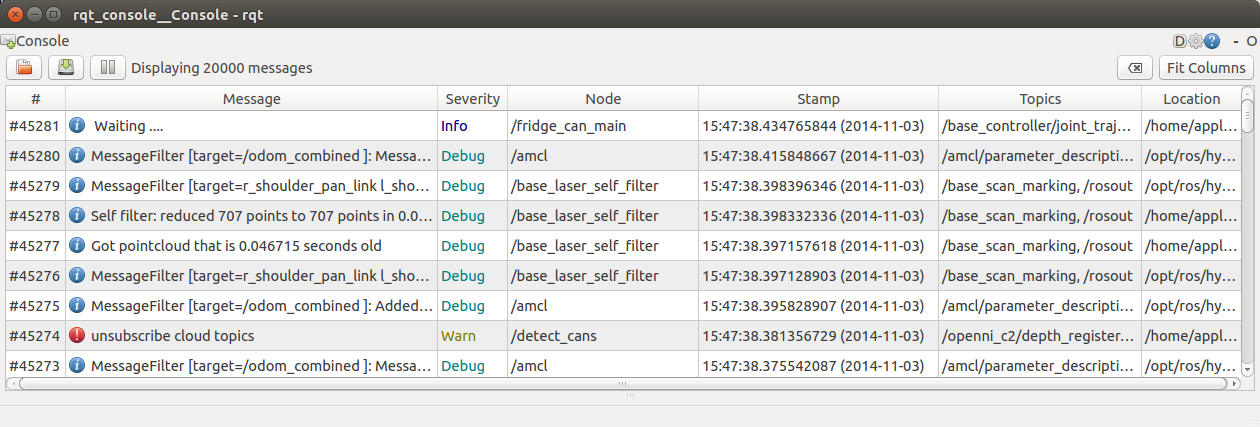
\includegraphics[width=0.6\columnwidth]{rqt_console.png}
\vspace*{-1mm}
\begin{nstabbing}
Us\=age:\\
\> \texttt{\$ rqt\_console}\\
\end{nstabbing}
\vspace*{-3mm}


\subsection{\href{http://wiki.ros.org/rqt_bag}{rqt\_bag}}
A tool for visualizing, inspecting, and replaying bag files.\\
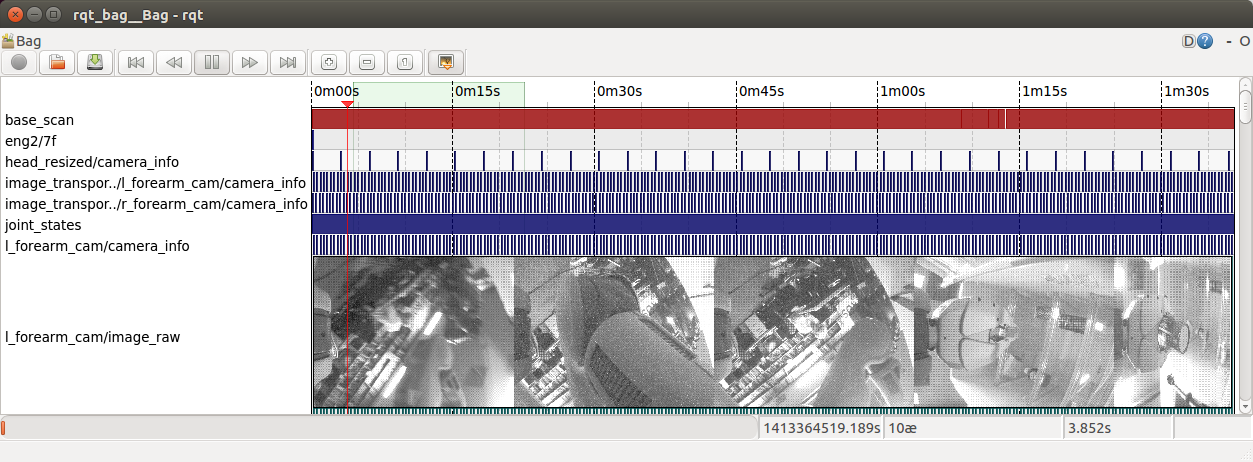
\includegraphics[width=0.6\columnwidth]{rqt_bag.png}
\vspace*{-1mm}
\begin{nstabbing}
Us\=age, viewing:\\
\> \texttt{\$ rqt\_bag bag\_file.bag}\\
Us\=age, bagging:\\
\> \texttt{\$ rqt\_bag *press the big red record button.*}\\
\end{nstabbing}
\vspace*{-3mm}

\subsection{\href{http://wiki.ros.org/rqt_logger_level}{rqt\_logger\_level}}
Change the logger level of ROS nodes. This will increase or decrease the information they log to the screen and rqt\_console.\\
\vspace*{-1mm}
\begin{nstabbing}
Us\=age:\\
\> \texttt{viewing \$ rqt\_logger\_level}\\
\end{nstabbing}
\vspace*{-3mm}

\section{Introspection \& Command Tools}
\vspace*{-1mm}

\subsection{\href{http://wiki.ros.org/rqt_topic}{rqt\_topic}}
A tool for viewing published topics in real time.\\
\vspace*{-1mm}
\begin{nstabbing}
Us\=age:\\
\> \texttt{\$ rqt}\\
\> \texttt{\footnotesize Plugin Menu->Topic->Topic Monitor}\\
\end{nstabbing}
\vspace*{-3mm}

\subsection{\href{http://wiki.ros.org/rqt_msg}{rqt\_msg}, \href{http://wiki.ros.org/rqt_srv}{rqt\_srv}, and \href{http://wiki.ros.org/rqt_action}{rqt\_action}}
A tool for viewing available msgs, srvs, and actions.\\
\vspace*{-1mm}
\begin{nstabbing}
Us\=age:\\
\> \texttt{\$ rqt}\\
\> \texttt{\footnotesize Plugin Menu->Topic->Message Type Browser}\\
\> \texttt{\footnotesize Plugin Menu->Service->Service Type Browser}\\
\> \texttt{\footnotesize Plugin Menu->Action->Action Type Browser}\\
\end{nstabbing}
\vspace*{-3mm}

\subsection{\href{http://wiki.ros.org/rqt_top}{rqt\_top}}
A tool for ROS specific process monitoring.\\
\vspace*{-1mm}
\begin{nstabbing}
Us\=age:\\
\> \texttt{\$ rqt}\\
\> \texttt{\footnotesize Plugin Menu->Introspection->Process Monitor}\\
\end{nstabbing}
\vspace*{-3mm}

\subsection{\href{http://wiki.ros.org/rqt_publisher}{rqt\_publisher}, and \href{http://wiki.ros.org/rqt_service_caller}{rqt\_service\_caller}}
Tools for publishing messages and calling services.\\
\vspace*{-1mm}
\begin{nstabbing}
Us\=age:\\
\> \texttt{\$ rqt}\\
\> \texttt{\footnotesize Plugin Menu->Topic->Message Publisher}\\
\> \texttt{\footnotesize Plugin Menu->Service->Service Caller}\\
\end{nstabbing}
\vspace*{-3mm}


\subsection{\href{http://wiki.ros.org/rqt_reconfigure}{rqt\_reconfigure}}
A tool for dynamically reconfiguring ROS parameters.\\
\vspace*{-1mm}
\begin{nstabbing}
Us\=age:\\
\> \texttt{\$ rqt}\\
\> \texttt{\footnotesize Plugin Menu->Configuration->Dynamic Reconfigure}\\
\end{nstabbing}
\vspace*{-3mm}

\subsection{\href{http://wiki.ros.org/rqt_graph}{rqt\_graph}, and \href{http://wiki.ros.org/rqt_dep}{rqt\_dep}}
Tools for displaying graphs of running ROS nodes with connecting topics and package dependancies respectively.\\
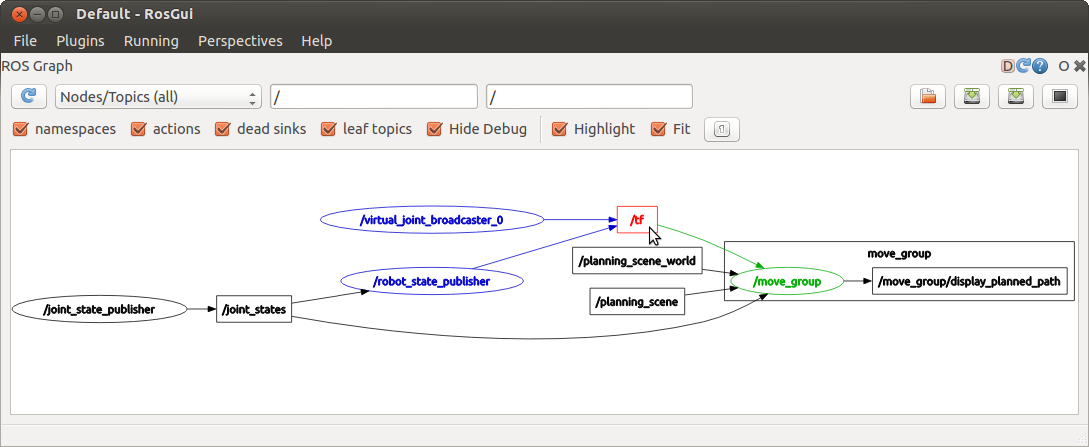
\includegraphics[width=0.45\columnwidth]{rqt_graph.png}
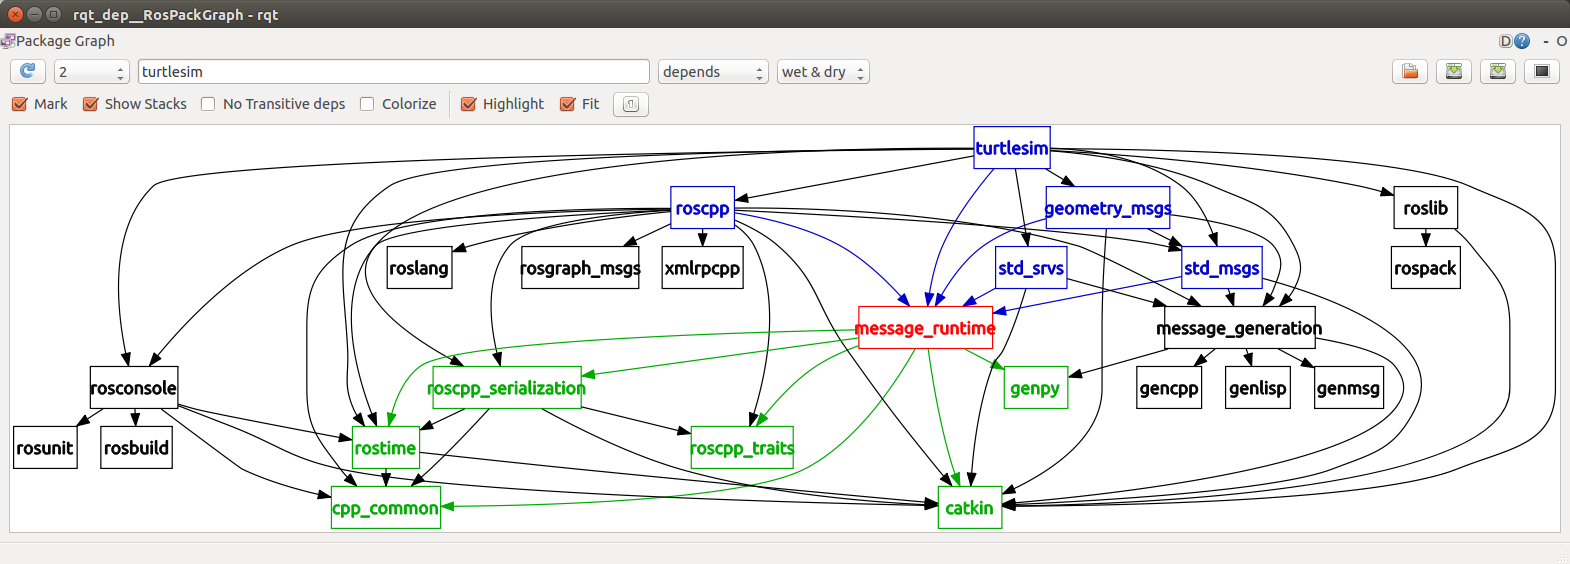
\includegraphics[width=0.53\columnwidth]{rqt_dep.png}
\vspace*{-3mm}
\begin{nstabbing}
Us\=age:\\
\> \texttt{\$ rqt\_graph}\\
\> \texttt{\$ rqt\_dep}\\
\end{nstabbing}
\vspace*{-3mm}



\section{Development Environments}

\subsection{\href{http://wiki.ros.org/rqt_shell}{rqt\_shell}, and \href{http://wiki.ros.org/rqt_py_console}{rqt\_py\_console}}
Two tools for accessing an xterm shell and python console respectively.\\
\vspace*{-1mm}
\begin{nstabbing}
Us\=age:\\
\> \texttt{\$ rqt}\\
\> \texttt{\footnotesize Plugin Menu->Miscellaneous Tools->Shell}\\
\> \texttt{\footnotesize Plugin Menu->Miscellaneous Tools->Python Console}
\end{nstabbing}
\vspace*{-1mm}

\section{Data Visualization Tools}

\subsection{\href{http://wiki.ros.org/tf2/Tutorials/Introduction to tf2\#Using_view_frames}{view\_frames}}
A tool for visualizing the full tree of coordinate transforms.\\
\vspace*{-1mm}
\begin{nstabbing}
Us\=age:\\
\> \texttt{\$ rosrun tf2\_tools view\_frames.py}\\
\> \texttt{\$ evince frames.pdf}
\end{nstabbing}
\vspace*{-2mm}


\subsection{\href{http://wiki.ros.org/rqt_plot}{rqt\_plot}}
A tool for plotting data from ROS topic fields.\\
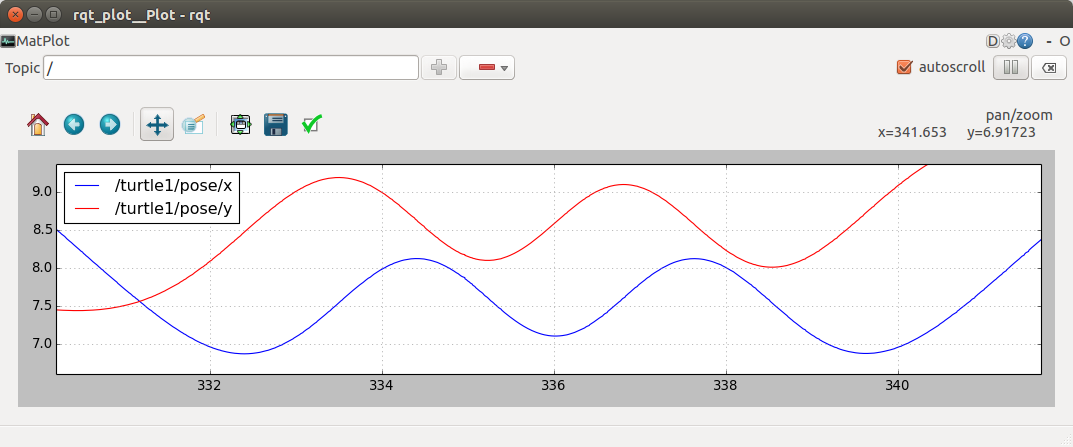
\includegraphics[width=0.6\columnwidth]{rqt_plot.png}
\vspace*{-1mm}
\begin{nstabbing}
E\=x\=amples:\\
\> To graph the data in different plots:\\
\> \>\texttt{\$ rqt\_plot /topic1/field1 /topic2/field2}\\
\> To graph the data all on the same plot:\\
\> \>\texttt{\$ rqt\_plot /topic1/field1,/topic2/field2}\\
\> To graph multiple fields of a message:\\
\> \>\texttt{\$ rqt\_plot /topic1/field1:field2:field3}\\
\end{nstabbing}
\vspace*{-2mm}

\vspace*{-2mm}
\subsection{\href{http://wiki.ros.org/rqt_image_view}{rqt\_image\_view}}
A tool to display image topics.\\
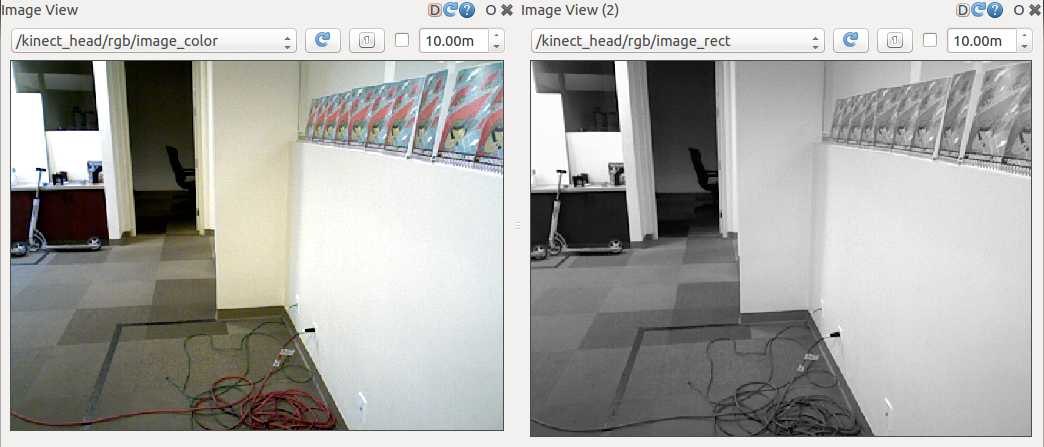
\includegraphics[width=0.5\columnwidth]{rqt_image_view.png}
\vspace*{-2mm}
\begin{nstabbing}
Us\=age:\\
\> \texttt{\$ rqt\_image\_view}\\
\end{nstabbing}
\vspace*{-2mm}


\vspace{1mm}
\ifcatkin
\section{ROS Indigo Catkin Workspaces}


\subsection{\href{http://wiki.ros.org/catkin/Tutorials/create_a_workspace}{Create a catkin workspace}}
Setup and use a new catkin workspace from scratch.
\begin{nstabbing}
E\=x\=ample:\\
\> \texttt{\$ source /opt/ros/indigo/setup.bash}\\
\> \texttt{\$ mkdir -p \textasciitilde/catkin\_ws/src}\\
\> \texttt{\$ cd \textasciitilde/catkin\_ws/src}\\
\> \texttt{\$ catkin\_init\_workspace}\\
\end{nstabbing}
\vspace{-3mm}

\subsection{\href{http://wiki.ros.org/catkin/Tutorials/CreatingPackage}{Checkout an existing ROS package}}
Get a local copy of the code for an existing package and keep it up to date using \href{http://wiki.ros.org/catkin/Tutorials/workspace\_overlaying}{wstool}.
\vspace{-1mm}
\begin{nstabbing}
E\=x\=amples:\\
\>\texttt{\$ cd \textasciitilde/catkin\_ws/src}\\
\>\texttt{\$ wstool init}\\
\>\texttt{\$ wstool set tut --git git://github.com/ros/ros\_tutorials.git}\\
\>\texttt{\$ wstool update}\\
\end{nstabbing}
\vspace{-3mm}



\subsection{\href{http://wiki.ros.org/catkin/Tutorials/CreatingPackage}{Create a new catkin ROS package}}

Create a new ROS catkin package in an existing workspace with \href{http://wiki.ros.org/catkin/Tutorials/CreatingPackage}{catkin create package}.% After using this you will need to edit the \href{http://wiki.ros.org/catkin/CMakeLists.txt}{CMakeLists.txt} to detail how you want your package built and add information to your \href{http://wiki.ros.org/catkin/package.xml}{package.xml}.
\vspace{-1mm}
\begin{nstabbing}
U\=sage:\\
\> \texttt{\$ catkin\_create\_pkg <package\_name> [depend1] [depend2]}\\
E\=x\=ample:\\
\> \texttt{\$ cd \textasciitilde/catkin\_ws/src}\\
\> \texttt{\$ catkin\_create\_pkg tutorials std\_msgs rospy roscpp}\\
\end{nstabbing}
\vspace{-3mm}

\subsection{\href{http://wiki.ros.org/catkin/Tutorials/using_a_workspace}{Build all packages in a workspace}}
Use \href{http://wiki.ros.org/catkin/Tutorials/using\_a\_workspace}{catkin\_make} to build all the packages in the workspace and then source the setup.bash to add the workspace to the \href{http://wiki.ros.org/ROS/EnvironmentVariables#ROS_PACKAGE_PATH}{ROS\_PACKAGE\_PATH}.
\vspace{-1mm}
\begin{nstabbing}
E\=x\=amples:\\
\> \texttt{\$ cd \textasciitilde/catkin\_ws}\\
\> \texttt{\$ \textasciitilde/catkin\_make}\\
\> \texttt{\$ source devel/setup.bash}\\
\end{nstabbing}
\vspace{-3mm}

%\vspace{-4.5 mm}
\subsection{\href{http://wiki.ros.org/catkin/CMakeLists.txt}{CMakeLists.txt}}
\vspace{-.5 mm}

\begin{tabbing}
Y\=our CMakeLists.tx\=t file MUST follow this format otherwise\\ your
packages will not build correctly.\\
\> \texttt{cmake\_minimum\_required()} Specify the name of the package\\
\> \texttt{project()} Project name which can refer as \$\{PROJECT\_NAME\}\\
\> \texttt{find\_package()} \> Find other packages needed for build\\
%\texttt{add\_message\_files(), add\_service\_files(), add\_action\_files()} & Message/Service/Action Generators\\
%\texttt{generate\_messages()} & Invoke message/service/action generation\\
\> \texttt{catkin\_package()} \> Specify package build info export\\
%\texttt{add\_library(), add\_executable(), target\_link\_libraries()} & Libraries/Executables to build\\
%\texttt{catkin\_add\_gtest()} & Tests to build\\
%\texttt{install()} & Install rules\\
\end{tabbing}
\vspace{-3.5mm}
\vspace{-2mm}
{\bf Build Executables and Libraries:}\\
Use CMake function to build executable and library targets. These
macro should call after \texttt{catkin\_package()} to use
\texttt{catkin\_*} variables.
\vspace{-3.5mm}
\begin{tabbing}
~ \texttt{include\_directories(include \$\{catkin\_INCLUDE\_DIRS\})}\\
~ \texttt{add\_executable(hoge src/hoge.cpp)}\\
~ \texttt{add\_library(fuga src/fuga.cpp)}\\
~ \texttt{target\_link\_libraries(hoge fuga \$\{catkin\_LIBRARIES\})}\\
\end{tabbing}
\vspace{-3.5mm}
\vspace{-2mm}
{\bf Message generation:}\\
%Your \texttt{package.xml} must contain a build and runtime dependency on
%\texttt{message\_generation} and \texttt{message\_runtime} respectively.
%There are \texttt{add\_message\_files(), add\_service\_files(),
%  add\_action\_files()} macros to handle messages,services and actions
There are \texttt{add\_\{message,service,action\}\_files()}
macros to handle messages,services and actions
respectively. They must call before \texttt{catkin\_package()}.
\vspace{-3.5mm}
\begin{tabbing}
~ \texttt{find\_package(catkin COMPONENTS message\_generation std\_msgs)}\\
~ \texttt{add\_message\_files(FILES Message1.msg)}\\
~ \texttt{generate\_messages(DEPENDENCIES std\_msgs)}\\
~ \texttt{catkin\_package(CATKIN\_DEPENDS message\_runtime)}\\
\end{tabbing}
\vspace{-5mm}
If your package builds messages as well as executables that use them,
you need to create an explicit dependency.
\vspace{-3.5mm}
\begin{tabbing}
~ \texttt{add\_dependencies(hoge \$\{PROJECT\_NAME\}\_generate\_messages\_cpp)}\\
\end{tabbing}

\vspace{-5mm}

%\vspace{30mm}
%\vspace{-10mm}

\else % \ifcatkin

\vspace{17cm}

\fi % \ifcatkin

%\begin{flushright}
%
\includegraphics[height=.12\columnwidth]{ros_logo.eps}
%\end{flushright}

\rule{0.3\linewidth}{0.25pt}

\scriptsize

Copyright \copyright\ 2015 Open Source Robotics Foundation

Copyright \copyright\ 2010 Willow Garage
%\vspace{3000 mm}


\end{multicols}
\end{document}
